\documentclass[12pt,journal]{IEEEtran}
\usepackage[
  backend=biber,
  style=numeric,
  citestyle=numeric
]{biblatex}
\usepackage{graphicx}
\addbibresource{citations.bib}
\providecommand{\keywords}[1]{\textbf{Keywords} #1}
\begin{document}
\title{Traffic Analysis on Tor}
\author{\IEEEauthorblockN{William Liddy\IEEEauthorrefmark{1}, Brian Pollack\IEEEauthorrefmark{2}}\\
        \IEEEauthorblockA{Department of Electrical Engineering and Computer Science\\Case Western Reserve University\\Cleveland, OH 44106\\\IEEEauthorrefmark{1}wjl36@case.edu, \IEEEauthorrefmark{2}bmp55@case.edu}}
\maketitle

\begin{abstract}
TODO: Abstract
\end{abstract}

% \keywords\\{TOR; Onion Routing, }

\section{Introduction}
\IEEEPARstart{T}{his} is the introduction.

\section{Background}
\subsection{Tor Architecture}
Tor is a circuit-based anonymous communication service that uses Onion Routing to securely pass packets in the network.
\par
A Tor circuit is the path that communication takes from the client to the desired destination. A circuit consists of multiple servers, called nodes, and is typically three nodes, or hops, long. To set up a circuit, the client must know the servers in which it would like to connect. The Tor network provides a list of appropriate nodes. The client then can send TCP packets through the circuit.
\par
Onion Routing is an overlay network protocol that is designed to carry TCP packets over existing networks. Traffic flows through the network in fixed size segments. Each node unwraps a layer from the packet using a symmetric key and forwards it to the next node. The packet is unwrapped like an union, which is where the name comes from.
\par
Tor routes its traffic using circuits. A user will set up a circuit using at least three Tor nodes, and that circuit stays active until the user either is finished or requests a new circuit. Tor circuits can carry any TCP packet, as long as the application supports routing through Tor, however cannot carry UDP packets. A single Tor circuit can carry multiple simultaneous streams, which is good for HTTP traffic which opens multiple connections to multiple destinations.
\par
One common attack against anonymous communication networks is known as traffic analysis. An attacker will analyze the traffic through a network to try to de-anonymize the users.
\par
While some anonymity services will reorder, mix, or otherwise shape the traffic flowing between Onion Routers, Tor chooses to not attempt to shape the traffic. The creators believed that all currently available traffic shaping strategies were still vulnerable to attacks and were difficult to implement practically. They also wanted to make Tor as low-latency as possible, and reordering packets would increase latency. Tor simply sends traffic in a round robin fashion.
\par
To protect against traffic bottlenecks, Tor uses a decentralized congestion control mechanism that sends end-to-end ack packets to maintain anonymity while allowing edge nodes to detect congestion and throttle their traffic until congestion subsides.
\par
Traffic is only allowed to leave the Tor network through nodes which specifically allow exits (called exit nodes). Each node has a policy stating which traffic is allowed to leave the network: this can be restricted by IP address or protocol. \cite{Dingledine:2004:TSO:1251375.1251396}

\subsection{Tor Threat Model}
Tor is designed to be impossible for attackers to link users with the services to which they are connecting \cite{Dingledine:2004:TSO:1251375.1251396}. The main goal of most attackers to the Tor network, therefore, is to de-identify its users and observe the remote services they are accessing. The attacker would then be limited by other encryption protocols, such as HTTPS, but that is beyond the scope of our study. A secondary goal of an attacker would be to group network connections, establishing a link among multiple connections to the same initiator. This would allow the attacker to build a profile on the user be observing with whom the user is communicating and by observing the user's communication habits \cite{Murdoch:2005:LTA:1058433.1059390}.
\par
If an attacker could identify individual users, this would constitute a major problem for Tor. If the entire point is to keep users anonymous, and it is proven that it is possible to de-anonymize certain users, the Tor network has significant problems that need to be addressed.
\par
Tor is designed to protect against an adversary who can observe some fraction of network traffic. This adversary can generate, modify, delete, or delay traffic and can operate his or her own tor nodes. The adversary can also compromise some fraction of existing tor nodes\cite{Dingledine:2004:TSO:1251375.1251396}.
\par
Additionally, it is important to note that Tor does not protect against traffic confirmation attacks, which are when an adversary suspects two parties are communicating and tries to prove it by analyzing the network. Tor rather attempts to make it difficult to identify who is communicating without a solid suspicion \cite{Murdoch:2005:LTA:1058433.1059390}.
\par
With our attacks, we try to gain information about the path of the Tor circuit using methods available to all Tor users. It is important to note that we do not exit the threat model for which Tor is built. We demonstrate that small attackers are able to gain insights about Tor users. This means that both government and non-government agencies are able to carry out these attacks on Tor.
\subsection{Tor Traffic Analysis}
Traffic analysis is the process of observing data from a network and making assumptions about users based on numerous properties such as the timing of packets or header information such as source and destination IP addresses. In the scope of anonymous networks, traffic analysis can be used with the goal of identifying end-users who are trying to remain anonymous \cite{Murdoch:2005:LTA:1058433.1059390}.
\par
On the Tor network, traffic analysis cannot be used to read the header information or content of the original TCP packets that are transmitted through the network while the packet is still in the Tor network. This type of traffic analysis can also be performed both before and after the original packet enters and leaves the Tor network, but that is beyond the scope of our threat model.
\par
Traffic analysis can be performed on the packets traveling through the Tor network. The attacker will not be able to read the header information or content of the original TCP packets because they are encased in the onion routing packets, but an attacker is able to gain information based on those onion routing packets.
\par
The type of traffic attacks which are most dangerous to the Tor network involve observing the traffic on a particular Tor node. Because Tor does not delay or reorder packets, we believe it to be susceptible to various types of traffic analysis attacks.
\par
Traffic analysis can be performed in multiple ways. An attacker can directly observe packets if he or she controls part of the network where the packets are flowing. Alternatively, an attacker can indirectly gain insights on a server by using measurements such as round trip time or a measurement of throughput on data through the server.
\par
We believe that if an attacker is observing a subset of nodes, he or she is able to effectively identify end-users through traffic analysis. Because we do not require a global observation of the network and do not require many Tor nodes under the attacker’s control, our network analysis attack is within the Tor threat model.


\begin{figure*}

 \center
  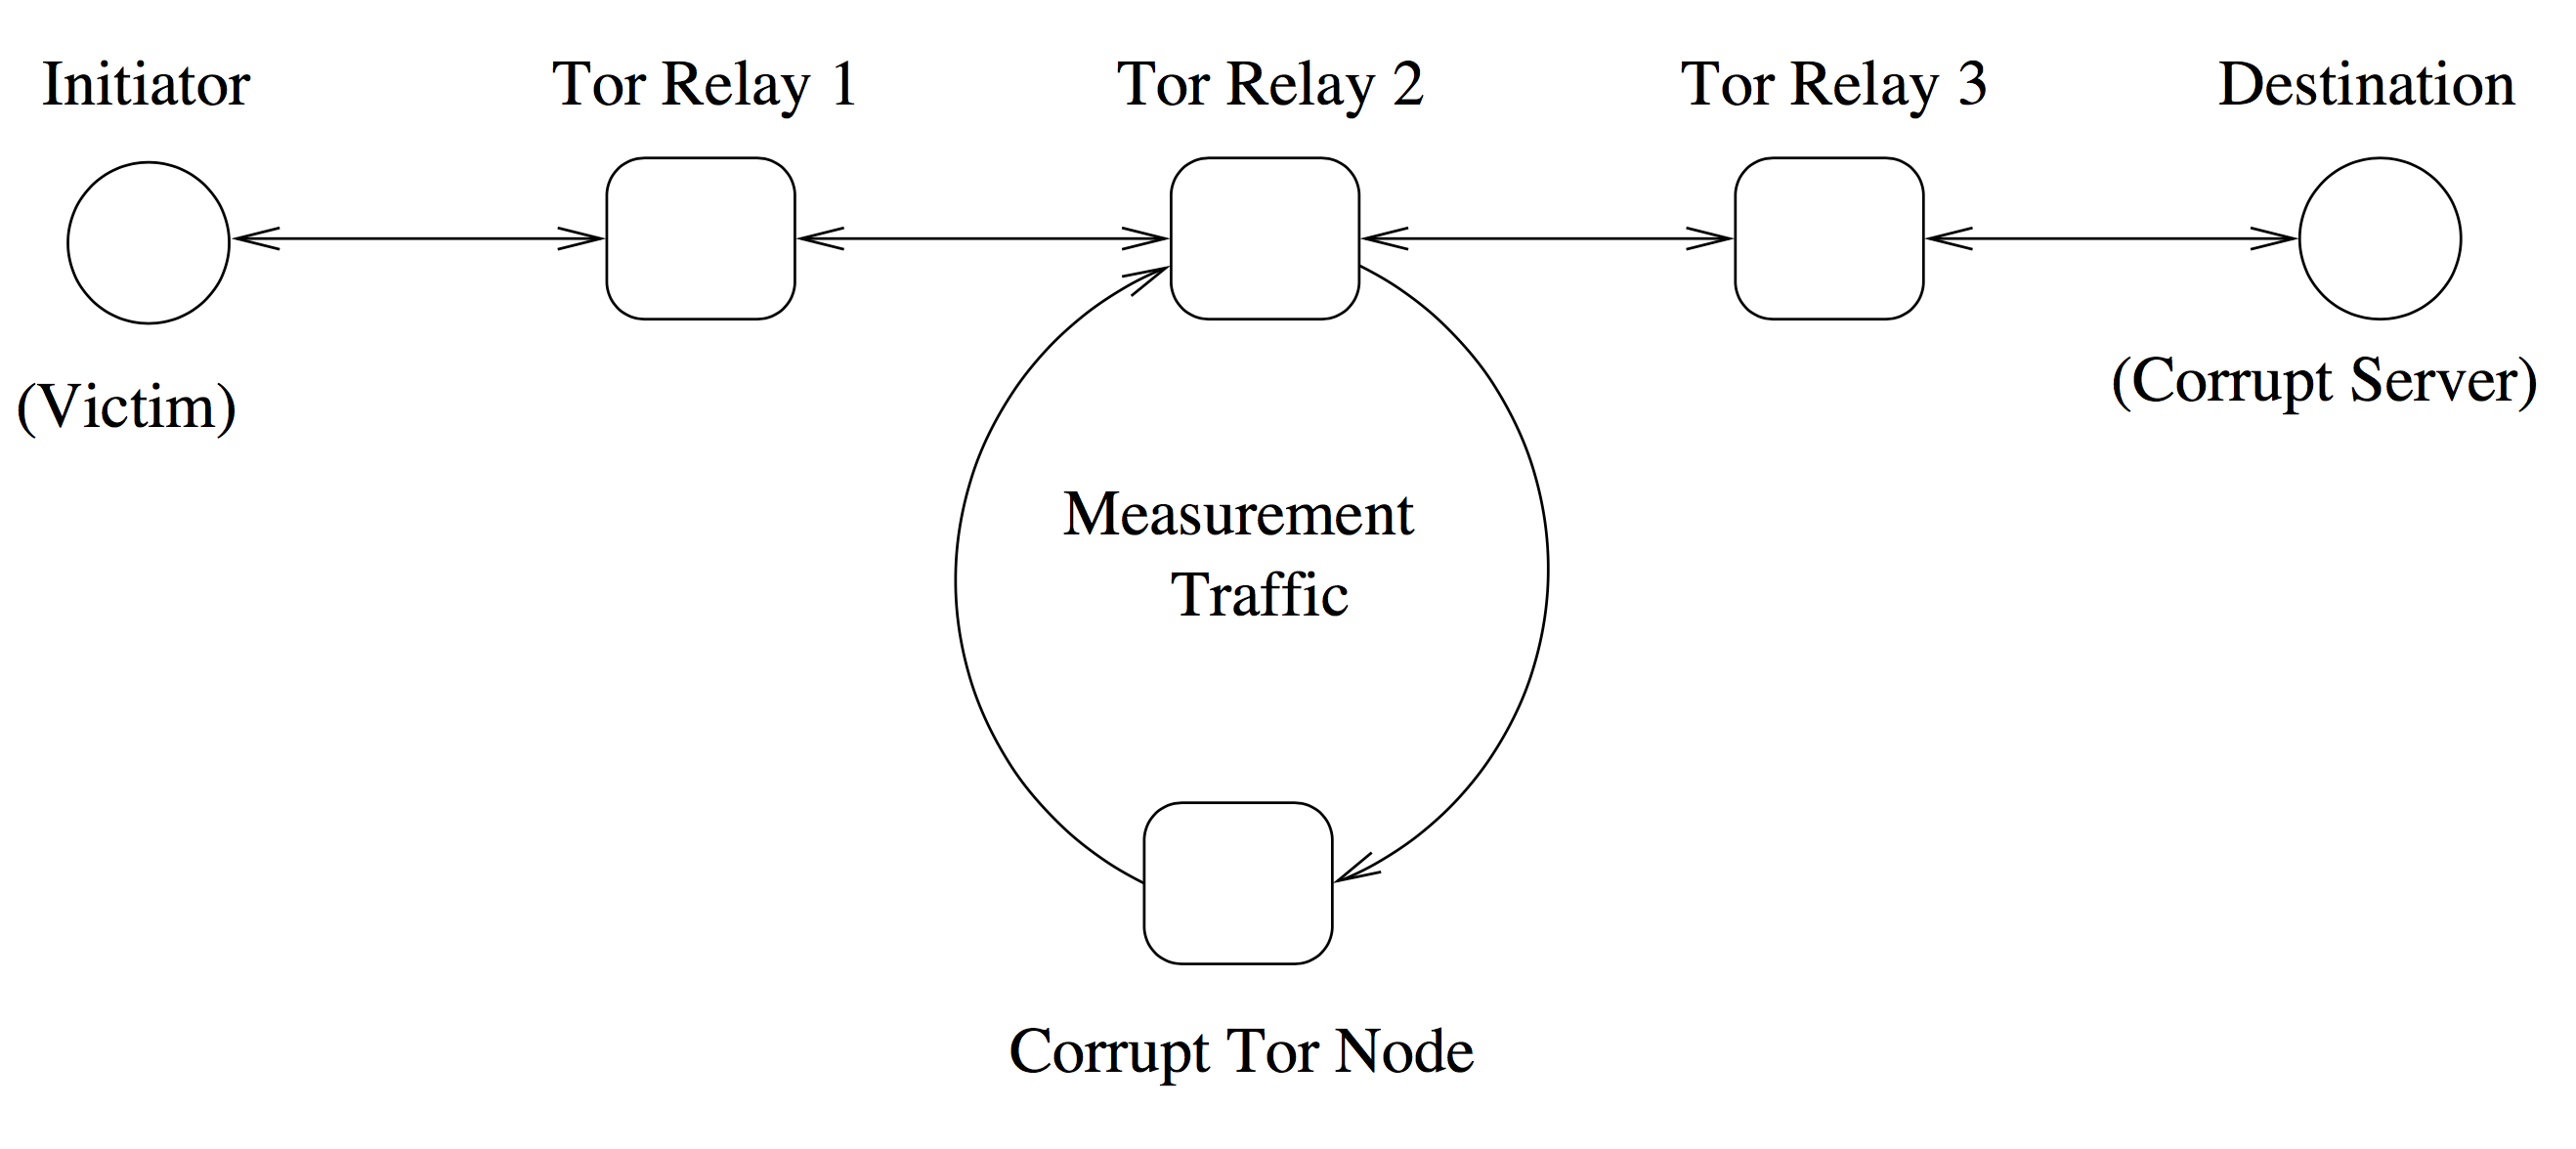
\includegraphics[width=\textwidth]{figures/murdochattacksetup.png}
  \caption{Murdoch and Danezis's Attack Setup \cite{Murdoch:2005:LTA:1058433.1059390}}
  \label{murdochsetup}
\end{figure*}

\subsection{Previous Work}
In 2005, Murdoch and Danezis studied similar attacks to the Tor network. They assumed that an adversary created a corrupt Tor node on the network. The corrupt node is then used to measure other nodes' traffic load. Additionally, they assumed that the attackers controlled a network server that the user to be traced is accessing. Murdoch and Danezis claim that this threat is within the threat model that should be covered by Tor. If the attackers modulate the data through the network server that the user is accessing, they were able to observe similar modulations in the Tor circuit that the user was using. This means, therefore, that the attackers could trace the user through the Tor circuit and link a user with the services he or she is using \cite{Murdoch:2005:LTA:1058433.1059390}. Figure \ref{murdochsetup} shows Murdoch and Danezis's attack setup.
\par
Because Murdoch and Danezis were able to observe the change in traffic patterns as users connected to a web service through a Tor circuit, they could infer which nodes were part of that circuit. This information by itself, however, does not seem too useful. At face value, we have identified servers through which a user is using to mask his or her traffic, but have not yet found that user. If we are the government or otherwise have access to the user's ISP, we can request logs of who is communicating with the servers in the Tor circuit and therefore can most likely identify the exact user who is trying to remain anonymous. This is disastrous in countries where the users are trying to remain anonymous due to government censorship as the government likely has access to this information.
\section{Our Setup and Results}
We wanted to test to see if the Tor network was still vulnerable to Murdoch and Danezis's attack. We did not simply duplicate their attack. Rather, we modified it slightly and reevaluated the exact attack scenarios. We wanted to demonstrate that this attack has significant real world implications that need to be addressed by the Tor network.
\subsection{Consensus Values}
When a Tor node is first created, it goes through four phases as it is being added to the Tor network. Each phase allows a different amount of traffic to be routed through the new node.
\subsubsection{Consensus Weight}
If anybody could immediately add a node to the Tor network and advertise that it can handle a large amount of traffic, other users would immediately start sending data through that new node. This means that an adversary could easily set up a node and allow many clients to set up circuits through it, then delay or drop those connections. It would be easy for adversaries to disrupt the Tor network. To combat this issue, Tor uses a measurement called consensus weight. Each client starts with a low consensus weight and, as other users send data through the new node, if the Tor network determines that the new node is performing well, the consensus weight will increase. The Tor network sends more traffic to nodes with a higher consensus weight.
\subsubsection{Guard Nodes}
On the Tor network, most clients build three hop curcuits. The very first Tor node with which a client interacts is slightly different than the rest because it helps protect the client against certain attacks. This first node is called a guard node. An anonymity attack that may be performed on the Tor network can look like this: if a client picks N paths at random, and an adversary controls a few Tor relays, then over time the chance that the client has made no connections through compromised Tor nodes goes to zero. The philosophy behind guard nodes is that the client will pick a guard node and will make every subsequent Tor circuit using that same guard node as the first hop. Either all of the client's connections will be compromised (the guard node will know the IP address of the client), or none of the client's connections will be compromised (each subsequent node in the circuit may know the guard node, but will never know the IP of the client). Once a Tor node is listed as a guard node, most clients will not use it as a middle node in a Tor circuit. This helps prevent the few nodes which are trusted as guard nodes from being overloaded \cite{arma2013}.
\subsubsection{Phase 1: unmeasured}
When a relay is first started, it will self-test its bandwidth. It publishes the results to its relay descriptor. For the first few days, the Tor network will allow only 20KB/s of bandwidth through the new node \cite{arma2013}.
\subsubsection{Phase 2: remote measurement}
After a few days, the new node will have received enough connections, despite its bandwidth being capped at 20KB/s, to begin to receive an increased consensus weight. When more traffic is received, if the node performs well enough, the consensus weight will be raised even more. During this phase, however, a node cannot be a guard node. The node will remain a middle node in the Tor network until moving on to phase three \cite{arma2013}.
\subsubsection{Phase 3: ramping up, guard relay}
To become a guard relay, a node must have a large enough consensus weight, a high enough uptime percentage, and a long enough time known to the Tor network. A node is eligible to become a guard node on the eigth day of its existance on the Tor network, assuming the first two conditions are satisfied. Over time, more and more clients will use the new node as a guard node and will remember that node to use for their next connections \cite{arma2013}.
\subsubsection{Phase 4: steady state, guard node}
Finally, once the new Tor relay has been a guard node for approximately twelve weeks, it will reach a steady state in which the number of new clients connecting to it as a guard node is equal to the number of clients who decide to choose a new guard node. This prevents the oldest guard nodes from becoming overloaded with traffic \cite{arma2013}.
\subsection{TORRC Configuration}
To configure the Tor service on a unix machine, the node operator has to modify the torrc configuration file. We just talked about the Tor service automatically ramping up bandwidth, but we point out that a node operator may choose to force the node to use a smaller bandwidth than his or her network will allow. An operator may choose to restrict bandwidth so the Tor node does not consume too much of the network.
\par
It is also worth stating that there are many other configuration options for the Tor service, and they are mostly located in the torrc configuration file. An operator can choose whether or not to allow the node to operate as a relay node or as an exit node and can set the ports that the tor service uses, among many other configuration options.
\subsection{Our Attack}
\begin{figure*}
 \center
  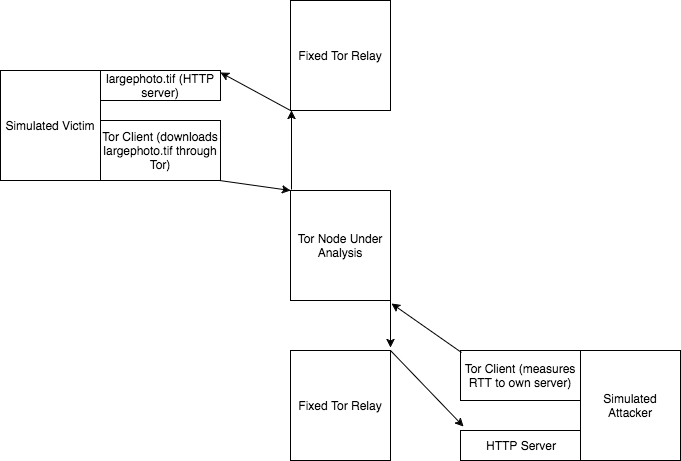
\includegraphics[width=\textwidth]{figures/oursetup.png}
  \caption{Our attack setup}
  \label{oursetup}
\end{figure*}
\subsubsection{Our Threat Model}
We begin with the assumption that a client will be accessing a service over the Tor network. We can also assume that an attacker has some control over and can generate, modify, delete, or delay traffic on either the client's network or the network of the web service. Lastly, we assume that the attacker has the ability to add a few nodes to the Tor network. All three of these assumptions are within the Tor threat model \cite{Dingledine:2004:TSO:1251375.1251396}.
To conduct our experiments, we first set up one Tor relay node and one Tor exit node, both using Lightsail on Amazon Web Services, and waited for them to be accepted to the Tor network.
\subsubsection{Our Victim}We then set up a victim machine which used the Tor network to download a large photo. The photo was hosted on an Apache webserver on the same machine as the victim client. The victim client used the Tor network to reach an arbitrary exit node which would then connect back to the webserver and download the image. The victim client was programmed to download the image for sixty seconds, then pause for sixty seconds, then repeat this process with a new Tor circuit.
\subsubsection{Our Analysis Node}The victim machine sent the fingerprints of the Tor nodes in each circuit it was using to our analysis node. The analysis node set up a Tor circuit through one of the nodes in the victim's circuit so it could try to detect that the client was using that node. We measured both the change in RTT and change in throughput through the analyzed node. See figure \ref{oursetup} for a diagram of our setup.
\subsubsection{Implications}
This setup is not unreasonable. We had three machines involved, including both the victim and analysis nodes. If the attacker has access to a victim's network, he or she could modulate the traffic by delaying packets, causing similar delays that we were using to experiment. If the attacker has access to the server to which the victim is connecting, the attacker can modulate the traffic there.
One additional way, which is the easiest for attackers to exploit, is for an attacker to interject his or her own content into the victim's connection by serving his or her modulated content on a legitimate website that the victim is accessing. For example, the simplest way of forcing the victim to download this modulated traffic is if the attacker purchased an advertisement on a website the victim was browsing. The attacker could then modulate the content that is downloaded by the client to load the advertisement.
Next, the attacker would need to have enough analysis nodes to be able to measure a significant percentage of the available Tor nodes. Because the attacker does not know any information about the victim's Tor circuit, he or she will need to analyze multiple nodes until the circuit is discovered. Especially if the search was limited to a subset of the active Tor nodes, we believe it is not unreasonable to assume that this attack is possible. The subset of measured nodes could start with all of the guard nodes, for example, which we know should constitute one hop in the victim's circuit.

\printbibliography
\end{document}
